\section{Iterative Co-Segmentation and Joint Registration}
\label{sec:segmentation}
如Figure~\ref{fig:iterative-segmentation-registration}所示展示了迭代分割与配准的系统流程。
\begin{figure*}
	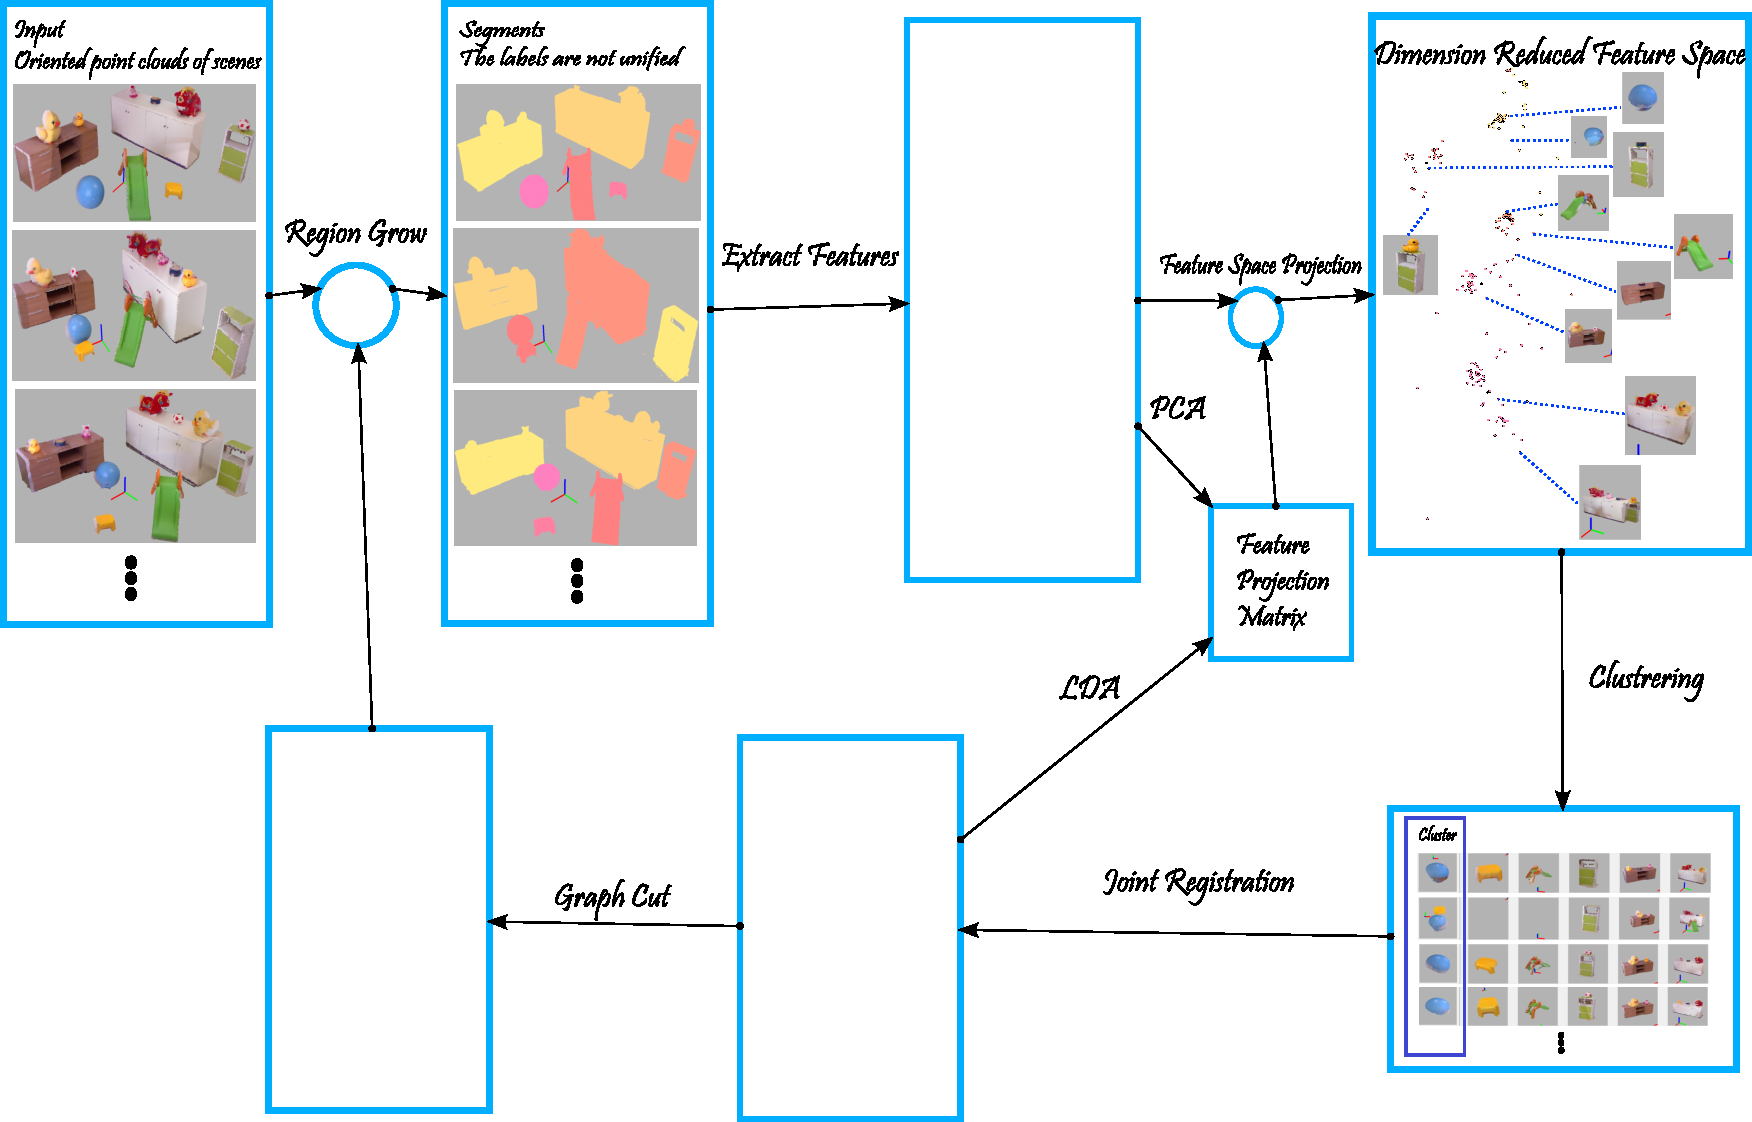
\includegraphics[width=1.0\textwidth]{figures/hsy/overview}
	\caption{Iterative co-segmentation and joint registration.}
	\label{fig:iterative-segmentation-registration}
\end{figure*}
\subsection{Region Grow}
区域生长的操作是对每一帧独立进行的。\\
输入是每一帧的点云以及每一帧所对应的label。\\
输出是更新之后的label。 \\
所谓label就是一个整数的数组它赋予点云中每一个点一个$id$,用来指示它所属的分割区域。我的实现中默认$id=0$的区域是未知区域(在图示中对应黑色区域)。在最开始时label的初始值是全为0。\\
区域生长操作是针对每一帧中的未知区域进行的,所使用的准则是如果两个区域之间有点互相在以R(默认$R=0.02$)为半径的邻域中就将这两个区域合并为同一个区域。\\
选择这样的准则基于的假设是相距较远且不连续的两组点云不太可能属于同一物体。\\
我们认为这样的准则会自然得到欠分割(under-segment)的分割结果。以便于后续能够进行配准(registration)操作\\
Figure~\ref{fig:object-iterations} 显示了第一次与第二次区域生长的过程。
\subsection{Object Clustering ( Unify Label )}
这一步操作是将每一帧的不同分割区域的patch无监督的聚成多个类以便于后续对每一类进行配准(registration)。
这一步输入是所有的点云以及它们对应的label,输出仍然是更新之后的label。
先依照前一步的label将点云分成多个patch,对所有的patch提取特征,然后依据投影矩阵将特征降维,然后再在低维空间中根据聚类中心为每一个patch重新分配id并更新每一帧的label。\\
关于使用了哪些特征?\\
如何得到投影矩阵?\\
如何确定聚类中心?\\
以下分别进行说明:
\subsubsection{Features}
Table~\ref{tab:features}列举了所有使用的特征以及对应的维数。
\begin{table}[!hbp]
\begin{tabular}{p{0.73\columnwidth}|{p{0.1\columnwidth}}}
\hline
Feature & Dimension\\
\hline
~\\
RGB Color Histogram & 125\\~\\
Size of Bounding Box & 3\\~\\
Percentage of Points Closest to Front-Back Left-Right Up-Down of its Bounding Box & 3\\~\\
Mean Distances to its Bounding Box ( Seperately Accounted for Front-Back Left-Right Up-Down  ) & 3 \\~\\
Standard Deviation of Distances to its Bounding Box ( Seperately Accounted for Front-Back Left-Right Up-Down  ) & 3
\end{tabular}
\caption{Patch Features} %表格的名称
\label{tab:features}
\end{table}
\subsubsection{Projection Matrix}
为什么降维,以及降维维数的选择:\\
1.将特征向量进行线性投影相当于为不同的特征赋予不同的权重来衡量。\\
2.之所以降维是为了后续能够进行k-means更新聚类中心。 k-means相当于一个简化的混合高斯的估计过程, 而要有效估计一个一维的高斯模型就按只需要五个样本(一般估计一个线性模型都至少要五个样本)来算,二维的要达到同样的采样密度需要25个样本,三维则需要至少125个样本。而我们的每组数据实际只有不到一百帧每个物体都没有125个这么多的样本。因此我认为降维到两维是合理的选择,同时这也方便对特征空间进行visualize。\\
降维的方法:\\
初始时投影矩阵是对所有patch的特征做PCA来生成的.
后续则根据配准的结果进行LDA来获得,使用LDA相当于学习一组新的特征权重来重新衡量。LDA获得的新的投影矩阵应会使得特征在新的子空间内的类内方差变小类间方差变大。类与类之间的可区分度更好。
具体的做法在章节~\ref{subsec:registration}中的对应小节中还会仔细说明。
\subsubsection{Cluster Centers}
聚类是在投影后的特征子空间内进行的,初始时候聚类中心是将patch最多的一帧的patch所对应的特征点作为聚类中心,然后进行k-means更新聚类中心。
再进行registration之后还会根据registration的结果再更新聚类中心。具体细节在具体的做法在章节~\ref{subsec:registration}中的对应小节中还会仔细说明。
\subsubsection{Cluster Assignment}
算法~\ref{alg:assignment}说明了根据聚类中心在特征子空间中为一帧中的每个patch指定类别的算法过程,目的在于要保证每一帧中最多有一个patch被指定到某个类别。
\begin{algorithm}[htb]
\caption{Assign Patch to Cluster}
\label{alg:assignment}
\textbf{Input:}~~\\
$\{P_i\}$:Patch Features of One Frame~~\\
$\{C_j\}$:Cluster Centers~~\\
\textbf{Output:}~~\\
$\{Id_i\}$:Identity for Each Patch in this Frame
\begin{enumerate}
\item Calculate Distance Matrix $D_{ij}:=d(P_i,C_j)$
\item Set Column Index $CIndex: = 1:J$
\item Set Row Index $RIndex: = 1:I$\\
\textbf{while} $D$ is not empty \textbf{do}
\item Find~~$(i,j)=min(D)$
\item Set $Id_{RIndex(i)}:=CIndex(j)$
\item Remove Row $i$ and Column $j$ from $D$
\item Remove Element $i$ from $RIndex$
\item Remove Element $j$ from $CIndex$\\
\textbf{end while}
\end{enumerate}
\end{algorithm}
\subsection{Joint Registration}
\label{subsec:registration}
联合配准的步骤参考\cite{Evangelidis-ECCV-2014}的算法把之前步骤中被分为同一类的patch进行配准,对于整个系统而言这一步主要起到以下几方面的作用:\\
1.为之前的聚类结果提供反馈。(更新特征投影矩阵和聚类中心)\\
2.建立起帧与帧之间的对应关系。为后续的联合分割能量项的生成提供桥梁。\\
3.在最后的迭代中配准生成的物体模型将作为结果输出。\\
\subsubsection{Update Cluster Centers}
图中第一行展示了几个有效的聚类中心在联合配准(joint registration)之后生成的物体模型,第二行中则展示了几个无效的聚类中心在联合配准之后生成的物体模型。
\subsection{Global Consistent Graph Cut}
\label{subsec:graphcut}

\begin{figure*}
\centering
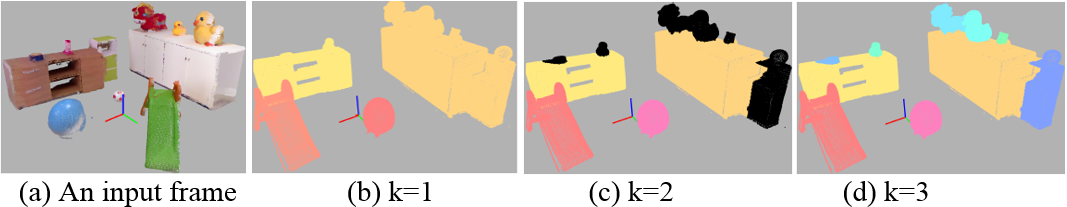
\includegraphics[width=2\columnwidth]{figures/object-iterations.png}
\caption{ The segmentation of each frame is progressively refined based on registered object models. From left to right: an input point cloud (a), segmentation updates at three iterations. \xj{show corresponding object model at each iteration.}}
\label{fig:object-iterations}
\end{figure*}
